
\pagestyle{empty}
\chapter*{\centering \large DAFTAR RIWAYAT HIDUP}
\thispagestyle{empty}
\onehalfspacing{}

\begin{wrapfigure}{l}{4cm}
	\vspace{-25pt}
	\begin{center}
		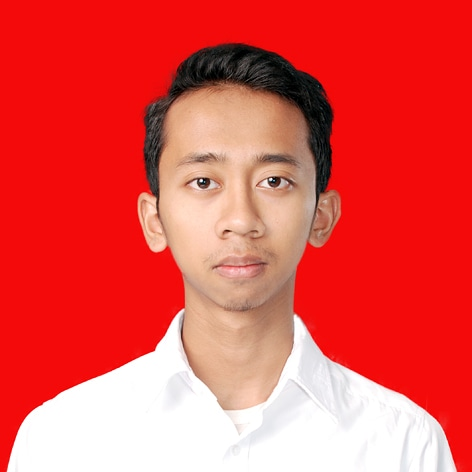
\includegraphics[width=0.27\textwidth]{gambar/pasfoto}
	\end{center}
	\vspace{-40pt}
\end{wrapfigure}

\noindent \textbf{MOCHAMMAD HANIF RAMADHAN.} Lahir di Jakarta, 25 Desember 1999.
Anak Kedua dari pasangan Bapak Akhadiyat Karsono dan Ibu Herlarti Kresnoyorini.
Saat ini penulis tinggal di Jl. Tembok Nomor 12 RT 002/RW 003, Kelurahan Kayu
Putih, Kecamatan Pulogadung, Kota Jakarta Timur, Provinsi DKI Jakarta.

\vspace{1cm}
\noindent
\begin{tabular}{lcl}
	No. Ponsel	& :&  081219853881 \\
	Email	& :&  hanifrmn@protonmail.com
\end{tabular}
\vspace{0.5cm}

\noindent \textbf{Riwayat Pendidikan} : Penulis mengikuti pendidikan sekolah
dasar di SD Islam Al-Azhar 13 Rawamangun pada tahun 2006 - 2012. Setelah itu,
penulis melanjutkan pendidikan di SMP Islam Al-Azhar 12 Rawamangun pada tahun
2012 - 2015. Kemudian penulis melanjutkan pendidikan di SMAN 68 Jakarta pada
tahun 2015 - 2018. Setelah lulus penulis sempat menjalani jenjang perkuliahan di 
Universitas Gunadarma pada tahun 2018, sebelum akhirnya melanjutkan perkuliahan 
di Universitas Negeri Jakarta pada tahun 2019.

\noindent \textbf{Riwayat Organisasi} : Selama di bangku perkuliahan, penulis 
terlibat dalam organisasi Badan Eksekutif Mahasiswa Program Studi Ilmu Komputer 
sebagai staff Departemen Akademik periode 2019-2020 dan Badan Eksekutif 
Mahasiswa Program Studi Ilmu Komputer sebagai kepala Departemen Akademik periode 
2020-2021. Penulis juga berpartisipasi dalam organisasi di lingkungan Program 
Studi Ilmu Komputer yaitu DEFAULT, di mana penulis membantu dalam upaya 
membangun ulang organisasi tersebut kembali.
